% !TEX encoding = UTF-8 Unicode
\documentclass[11pt,spanish]{article}\usepackage[]{graphicx}\usepackage[]{color}
% maxwidth is the original width if it is less than linewidth
% otherwise use linewidth (to make sure the graphics do not exceed the margin)
\makeatletter
\def\maxwidth{ %
  \ifdim\Gin@nat@width>\linewidth
    \linewidth
  \else
    \Gin@nat@width
  \fi
}
\makeatother

\definecolor{fgcolor}{rgb}{0.345, 0.345, 0.345}
\newcommand{\hlnum}[1]{\textcolor[rgb]{0.686,0.059,0.569}{#1}}%
\newcommand{\hlstr}[1]{\textcolor[rgb]{0.192,0.494,0.8}{#1}}%
\newcommand{\hlcom}[1]{\textcolor[rgb]{0.678,0.584,0.686}{\textit{#1}}}%
\newcommand{\hlopt}[1]{\textcolor[rgb]{0,0,0}{#1}}%
\newcommand{\hlstd}[1]{\textcolor[rgb]{0.345,0.345,0.345}{#1}}%
\newcommand{\hlkwa}[1]{\textcolor[rgb]{0.161,0.373,0.58}{\textbf{#1}}}%
\newcommand{\hlkwb}[1]{\textcolor[rgb]{0.69,0.353,0.396}{#1}}%
\newcommand{\hlkwc}[1]{\textcolor[rgb]{0.333,0.667,0.333}{#1}}%
\newcommand{\hlkwd}[1]{\textcolor[rgb]{0.737,0.353,0.396}{\textbf{#1}}}%
\let\hlipl\hlkwb

\usepackage{framed}
\makeatletter
\newenvironment{kframe}{%
 \def\at@end@of@kframe{}%
 \ifinner\ifhmode%
  \def\at@end@of@kframe{\end{minipage}}%
  \begin{minipage}{\columnwidth}%
 \fi\fi%
 \def\FrameCommand##1{\hskip\@totalleftmargin \hskip-\fboxsep
 \colorbox{shadecolor}{##1}\hskip-\fboxsep
     % There is no \\@totalrightmargin, so:
     \hskip-\linewidth \hskip-\@totalleftmargin \hskip\columnwidth}%
 \MakeFramed {\advance\hsize-\width
   \@totalleftmargin\z@ \linewidth\hsize
   \@setminipage}}%
 {\par\unskip\endMakeFramed%
 \at@end@of@kframe}
\makeatother

\definecolor{shadecolor}{rgb}{.97, .97, .97}
\definecolor{messagecolor}{rgb}{0, 0, 0}
\definecolor{warningcolor}{rgb}{1, 0, 1}
\definecolor{errorcolor}{rgb}{1, 0, 0}
\newenvironment{knitrout}{}{} % an empty environment to be redefined in TeX

\usepackage{alltt}
\usepackage[spanish,mexico]{babel}
\usepackage[utf8]{inputenc}
\usepackage{authblk}
\usepackage{setspace}
\usepackage[margin=1in]{geometry}
\usepackage{graphicx}
\usepackage{subcaption}
\usepackage{amsmath}
\usepackage[table,xcdraw]{xcolor}
\usepackage[rightcaption]{sidecap}
\usepackage[colorlinks = true,
            linkcolor = black,
            urlcolor  = gray,
            citecolor = black,
            anchorcolor = black]{hyperref}

\usepackage{natbib}
\bibliographystyle{apalike}

\usepackage{booktabs}
\usepackage[table,xcdraw]{xcolor}

\let\olditemize\itemize
\def\itemize{\olditemize\itemsep=0pt}

%%%%%% Title %%%%%%
% Full titles can be a maximum of 200 characters, including spaces. 
% Title Format: Use title case, capitalizing the first letter of each word, except for certain small words, such as articles and short prepositions
\title{\huge{Reporte de trabajo: Análisis de Redes con datos del Tamizaje para la detección de riesgos a la Salud Mental por Covid-19}}

%%%%%% Authors %%%%%%
\author[ ]{Elena Villalobos Nolasco}

%%%%%% Date %%%%%%
% Date is optional
\date{Enero, 2022.}

%%%%%% Spacing %%%%%%
% Use paragraph spacing of 1.5 or 2 (for double spacing, use command \doublespacing)
\onehalfspacing
\IfFileExists{upquote.sty}{\usepackage{upquote}}{}
\begin{document}

\maketitle

%%%%%% Main Text %%%%%%

El presente documento tiene los avances realizados en el proyecto de {\bf Análisis de Redes como alternativa de análisis para estudiar psicopatologías}\footnote{Todo el código e información asociada a este proyecto se encuentra en el siguiente repositorio: \url{https://github.com/ElenaVillano/mental_networks}} y tiene como base principal el tutorial de \cite{main_tutorial} y sus materiales adicionales \citep{epskamp2018estimating}. En la primera parte del documento hablaremos de los conceptos básicos para entender el análisis de redes, así como de la descripción de los gráficos principales para estudiar las características de las redes. En la segunda parte, presentaremos algunos resultados obtenidos de la base de datos del Tamizaje para la detección de riesgos a la Salud Mental por Covid-19 \citep{morales2021mental, chaine2020condiciones}. 


\section{Conceptos básicos para entender el análisis de redes}

El análisis de redes, basado en la teoría de grafos, es un método analítico que tiene como objetivo estudiar las interrelaciones existentes entre entidades. En éste, los nodos representan entidades (aeropuertos, personas, etc.), y las conexiones, también conocidas como aristas, son observadas, medidas y conocidas (número de vuelos entre aeropuertos, amistades, etc.). Además, en el análisis de redes, las aristas puedes ser dirigidas o no dirigidas, en las primeras hay un nodo de origen y un nodo destino, en las segundas una arista representa una conexión simétrica entre dos nodos. Para este estudio se utilizarán redes no dirigidas que representan una relación entre los nodos. 

De manera similar pero estructuralmente diferente al análisis de redes, las redes psicológicas consisten en nodos que representan las variables observadas que están interconectados por aristas que representan relaciones estadísticas, las cuales se infieren a partir de los mismos datos. Por ejemplo, en un cuestionario psicométrico las respuestas a las preguntas de presencia/ausencia de síntomas son los nodos, y lo que se infiere son interrelaciones entre los nodos o síntomas. Como dichas interrelaciones se estiman a partir de los datos, es muy recomendable tener más datos que ayuden a hacer cómputos más confiables.

A grandes rasgos, el análisis de redes psicológicas tiene dos pasos involucrados:

\begin{enumerate}
  \item Estimar el modelo estadístico sobre los datos, es decir, la estimación de la red con sus pesos correspondientes entre las variables observadas. 
  \item Analizar si las estimaciones de los pesos de la red son adecuadas, a partir de medidas desarrolladas en teoría de grafos. 
\end{enumerate}

De manera específica, en las redes psicológicas {\bf los nodos representan las variables observadas y las aristas representan coeficientes de correlación parcial entre variables (i.e. pesos de las aristas), condicionadas sobre las otras variables observadas}. 

En toda red estimada, se tiene que valorar la importancia o conectividad de los nodos dentro de la red, para lo que se computan las medidas de centralidad \citep{felipe} que son: 

\begin{description}
  \item[Fuerza del nodo:] que tan bien el nodo esta {\bf directamente} conectado con otros nodos. Una manera de interpretarlo, es qué tan importante es el nodo dentro de la red conectando directamente con otros nodos. 
  \item[Cercanía o closeness:] cuantificar que tan bien el nodo es indirectamente conectado a otros nodos. Es una especie de promedio que nos dice qué tan lejos están los otros nodos de la red. 
  \item[Intermediación o betweeness:] que tan importante es un nodo en el camino promedio entre dos nodos. Otra manera de decirlo es qué tan único es el nodo para conectar con otros pares de nodos de la red. 
\end{description}

Dentro del tutorial de \cite{main_tutorial}, simularon una red con un modelo gráfico gausiano del cual obtuvieron las medidas de centralidad ya descritas, ambos presentados en la Figura \ref{fig:tuto_red}. La red la estimaron utilizando una base de datos donde cada uno de los 17 reactivos, hablaban de síntomas de estrés post-traumático. En ésta se puede observar de lado izquierdo que las conexiones más fuertes positivas son entre los nodos o síntomas 16 y 17, 3 y 4, y 11 y 5, pues entre más concentración de color y grosor en la arista, más correlación positiva parcial hay entre esos nodos. De la misma manera, se puede observar una relación negativa delgada entre los nodos 10 y 12, representada por la presencia del color rojo. También, la ausencia de conexión entre los nodos es indicio de que hay independencia estadística (no hay relación) entre los nodos cuando se condiciona sobre los otros síntomas. En cuanto a las medidas de centralidad en el panel derecho, el nodo 17 y el 3 salen como los más importantes para la red, tanto para la fuerza del nodo como para \emph{betweenness}. 

\begin{figure}[!ht]
\centering
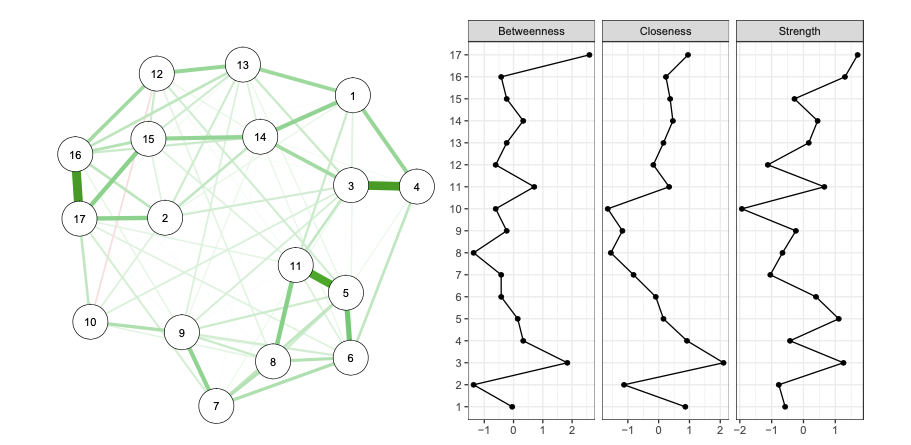
\includegraphics[scale=0.5]{images/red_medidas_tutorial}
\caption{Red de modelo gráfico gausiano del cuestionario PTSD con 17 reactivos (panel izquierdo) y sus respectivos índices de centralidad (panel derecho), presentados en el tutorial de \cite{main_tutorial}}.
\label{fig:tuto_red}
\end{figure}

A partir de los parámetros obtenidos del modelo anterior se simularon datos de 500 sujetos más. Se observó que la red que se generó era muy similar a la original. Sin embargo, se encontró que las medidas de centralidad difieren mucho entre las simulaciones y el modelo original. Por lo que destacaron la importancia de evaluar la precisión de las estructuras de las redes psicológicas, y para ello sugieren los siguientes tres pasos: 

\begin{enumerate}
  \item Estimar la precisión de los pesos de las aristas, utilizando Intervalos de Confianza con bootstrap.
  \item Evaluar la estabilidad de los índices de centralidad observados sobre sub-conjuntos de datos.
  \item Realizar tests de diferencias significativas entre los pesos de las aristas y los índices de centralidad. 
\end{enumerate}

Antes de presentar la evaluación de la precisión de las redes, en la siguiente sección destacaremos algunas partes importantes sobre el análisis de redes.

\subsection*{Especificaciones de estimaciones de redes psicológicas.}

Un modelo de redes que se usa popularmente para estimar redes psicológicas es un Campo Aleatorio de Markov por Pares (Pairwise Markov Random Field, PMRF). En este modelo, los nodos representan variables, y se conectan a través de aristas no-direccionadas, indicando dependencia condicional entre dos variables; dos variables que no están conectadas son independientes después de condicionar sobre las otras variables. Cuando los datos son normales multivariados, esta independencia condicional correspondería a una correlación parcial igual a cero. De manera específica, los parámetros de los pesos de las aristas se interpretan como la fuerza de asociaciones únicas entre variables, que {\bf pueden} indicar potenciales relaciones causales. 

Cuando los datos son binarios, el modelo PRMF a utilizar es el modelo Ising. Mientras que si los datos siguen una densidad normal multivariada, el modelo apropiado de PRMF es el modelo gráfico gausiano (GGM), en el que las aristas pueden ser directamente interpretadas como coeficientes de correlación parcial. El GGM requiere un estimado de la matriz de covarianza como entrada, que en caso de que los datos sean ordinales se pueden utilizar correlaciones policóricas (i.e. correlación para variables ordinales de variables latentes).

El modelo PMRF tiene el problema de que el número de parámetros a estimar crece mucho con el tamaño de la red y en generalmente en el área de psicología no se tienen tantos datos que compensen esta sobre-estimación. Para tratar dicho problema se utiliza la forma de regularización de LASSO (Least Absolute Shrinkage and Selection Operator), técnica penaliza el uso de muchos parámetros, limitando la suma de valores paramétricos absolutos. Por lo que LASSO regresa un modelo de red más conservador, que en otras palabras, sólo un pequeño número de aristas se utilizan para explicar la covariación de la estructura en los datos\footnote{El paquete de \texttt{qgraph} \citep{packageqgraph, bootnet} utiliza lasso en combinación con la selección de modelos EBIC para estimar un GGM regularizado.}. 


\subsection{Precisión de los pesos de las aristas}

Para evaluar la variabilidad de los pesos de las aritas se pueden estimar Intervalos de Confianza\footnote{Para construir Intervalos de Confianza se necesita saber la \emph{distribución muestral} del estadístico de interés. Sin embargo, saber dicha distribución para medidas de centralidad, es difícil por su misma complejidad de cómputo. Por lo que se utiliza bootstrap, que es una técnica que implica estimar repetidamente un modelo con datos muestreados o simulados para obtener el estadístico de interés. Se puede hacer bootstrap de dos maneras, paramétrico y no parámetrico. En el \emph{no paramétrico}, las observaciones de los datos se re-muestrean con reemplazo para crear un nuevo conjunto de datos, mientras que el \emph{paramétrico} muestrea nuevas observaciones del modelo paramétrico que fue estimado a partir de los datos originales, lo que crea una serie de valores que pueden ser utilizados para estimar la distribución muestral.} con la técnica de re-muestreo bootstrap. Se aconseja que para datos ordinales, se utilice bootstrap no paramétrico. 

Es importante mencionar que los resultados del bootstrap no deberían ser utilizados para hacer test de significancia diferente de cero, pues la regularización de LASSO ayuda a quitar los pesos que no son importantes en la red. Esto significa que los pesos que aparecen dentro de la red, ya pueden ser significativamente diferentes de cero, por lo que conviene considerarlos como importantes. 

Entonces la interpretación de los Intervalos de Confianza con bootstrap para los pesos de las aristas no se deben asumir diferentes de cero, si no que sólo muestran la precisión de esos pesos y lo que se debe de hacer es comparar los valores de las aristas entre ellos. Cuando un intervalo es ancho, es difícil hacer la interpretación de la fuerza del nodo, por lo que probablemente resultará en poca precisión para las otras medidas de centralidad. 

La Figura \ref{fig:inter_boot_tutorial}, son los Intervalos de Confianza para el modelo presentado al inicio de este documento (figura \ref{fig:tuto_red}). En este gráfico cada línea horizontal representa una arista de la red, ordenadas desde la arista con el peso más alto, hasta la arista con el peso más bajo. Es decir, las conexiones colocadas en la parte superior del gráfico son las más fuertes, que son entre los nodos 17 y 16, 3 y 4, y 11 y 5. Se podría considerar que son, de manera confiable, las tres aristas con más fuerza de conexión debido a que sus Intervalos de Confianza no se superponen con los intervalos de ninguna otra arista.

\begin{figure}[!ht]
\centering
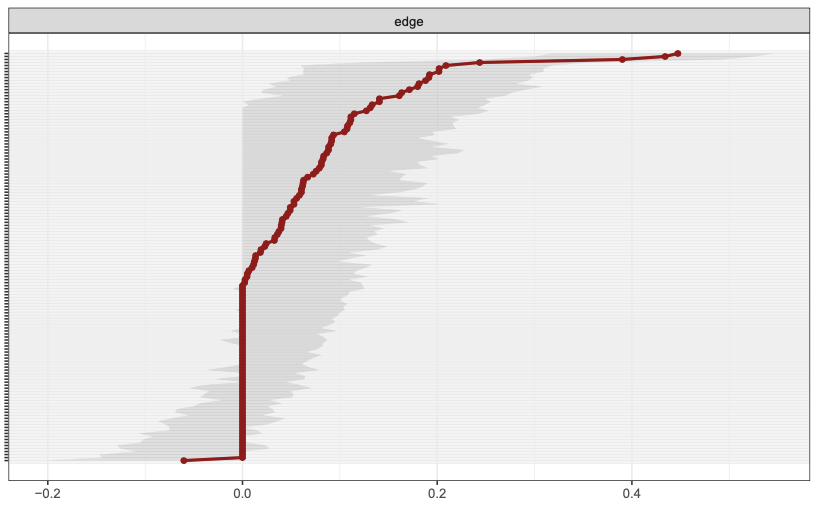
\includegraphics[scale=0.5]{images/intervalos_boot_tutorial}
\caption{Intervalos de Confianza bootstrap de \cite{main_tutorial}.}
\label{fig:inter_boot_tutorial}
\end{figure}

\subsection{Estabilidad de centralidad}

Para saber la estabilidad de las medidas de centralidad no se puede utilizar bootstrap\footnote{Esto es porque se generan distribuciones muestrales sesgadas.}, por lo que se propone estudiar dichas medidas con subconjuntos de datos. Se dice que los índices de centralidad son estables cuando el orden de los índices es el mismo en diferentes sub-muestras del mismo conjunto de datos. Lo que se hace es que se aplica la técnica de re-muestreo (el bootstrap regular) para diversas proporciones de los mismos participantes (o variables) y se evalúa si la correlación entre los índices de centralidad originales y aquellos obtenidos en las sub-muestras, son estables. Si la correlación cambia completamente después de quitar 10\% de la muestra, por ejemplo, entonces las interpretaciones de centralidad pueden ser erróneas. A esto se le llama bootstrap de subconjuntos con \emph{case-dropping}. Para cuantificar dicha estabilidad se propone la medida de coeficiente de estabilidad de correlación (CS-coefficient), que se recomienda sea mayor a 0.7.


La Figura \ref{fig:estabilidad_tutorial}, muestra la estabilidad de las medidas de centralidad del modelo que se ha venido presentando. Éste debe de permanecer estable y tener promedio de correlación similar entre los diferentes porcentajes de muestra. Por lo tanto, se espera que las líneas se mantengan rectas y en la parte superior a lo largo de los porcentajes que están en el eje x. Para este caso, la medida de fuerza parece ser la más estable, mientras que \emph{betweennes} y \emph{closeness}, tienen mayor disminución conforme se reduce el porcentaje de muestra. 

\begin{figure}[!ht]
\centering
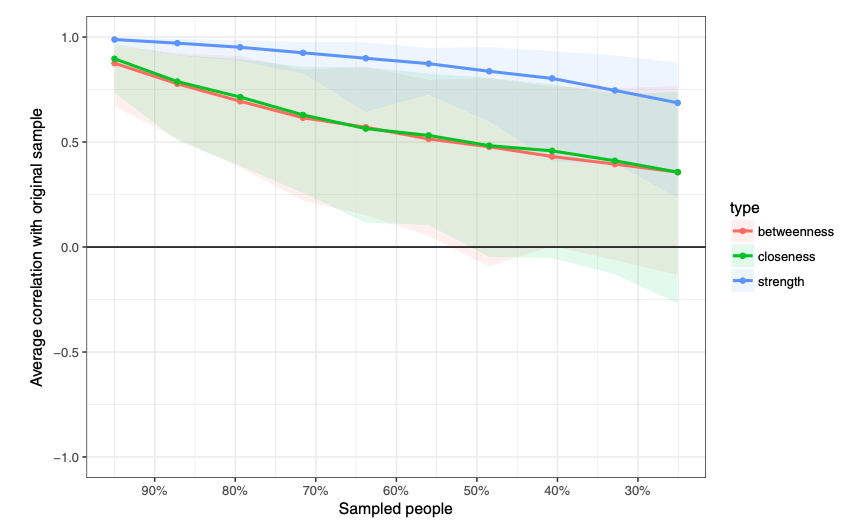
\includegraphics[scale=0.5]{images/estabilidad_tutorial}
\caption{Estabilidad de las medidas de centralidad del ejemplo \cite{main_tutorial}.}
\label{fig:estabilidad_tutorial}
\end{figure}

\subsection{Test para diferencias significativas}

El test de diferencias significativas, que también se hace con bootstrap, se utiliza para saber si una arista es significativamente distinta de otra, o si las medidas de centralidad de los nodos son significativamente distintas de otros nodos. En este test se recomienda, tener cuidado en la interpretación debido a que el no rechazar la hipótesis nula, no es evidencia de que la hipótesis alternativa sea verdadera\footnote{Hipótesis nula: no hay diferencias.}. Para este tipo de gráficos que se presenta una matriz cuadrada, en donde los cuadros negros representan diferencia significativa entre los pares que se indiquen en los ejes $x$ y $y$, y los grises son diferencias no son significativas. En la siguiente sección de resultados presentaremos un gráfico como el que se menciona. 

\newpage

\section{Resultados}

En esta sección se hablará de tres modelos de redes que se crearon a partir del Tamizaje para la detección de riesgos a la Salud Mental por Covid-19, con 102,209 participantes. Para el presente análisis sólo se usaron preguntas referentes a síntomas de depresión, ansiedad, estrés, etc. Los reactivos que se utilizaron se basan en cuestionarios psicométricos como el PCL-5 que es para estrés postraumático, y el GAD-7 que es para ansiedad generalizada. Cada respuesta va de 0 al 10, donde cero es nada y 10 es extremo; la tabla \ref{tab:tablareactivos} presenta una breve descripción de cada reactivo. 
\vspace{0.5cm}

% Please add the following required packages to your document preamble:
% \usepackage[table,xcdraw]{xcolor}
% If you use beamer only pass "xcolor=table" option, i.e. \documentclass[xcolor=table]{beamer}
\begin{table}[h]
\centering
\begin{tabular}{|c|l|c|}
\hline
\rowcolor[HTML]{EFEFEF} 
ID & \multicolumn{1}{c|}{\cellcolor[HTML]{EFEFEF}Variable} & Constructo \\ \hline
\begin{tabular}[c]{@{}c@{}}st1\\ st2\\ st3\\ st4\\ st8\\ st12\\ st17\end{tabular} & \begin{tabular}[c]{@{}l@{}}Pienso/imagino enfermar\\ Pesadillas sobre enfermar\\ Preocupación por mención enfermedad\\ Reacciones físicas al pensar en enfermar\\ Si alguien enferma es por mi culpa\\ Incertidumbre de futuro por enfermedad\\ Asustado por padecer enfermedad\end{tabular} & Estrés \\ \hline
\begin{tabular}[c]{@{}c@{}}av5\\ av6\\ av7\end{tabular} & \begin{tabular}[c]{@{}l@{}}Evito pensar/hablar sobre enfermedad\\ Evito escuchar fuentes oficiales sobre enfermedad\\ Dificultad para recordar recomendaciones oficiales\end{tabular} & Evitación \\ \hline
\begin{tabular}[c]{@{}c@{}}d9\\ d10\\ d11\\ d13\\ d14\\ d15\\ d16\end{tabular} & \begin{tabular}[c]{@{}l@{}}He perdido interés por actividades \\ Distante con personas que convivo \\ Dificultad de afecto por seres queridos\\ Deseo de hacerme daño\\ Dificultad para dormir o seguir dormido\\ Me siento enojado\\ Me cuesta trabajo poner atención\end{tabular} & Distanciamiento \\ \hline
\begin{tabular}[c]{@{}c@{}}ag18\\ ag19\\ ag20\\ ag21\\ ag22\end{tabular} & \begin{tabular}[c]{@{}l@{}}Me siento ansioso/nervioso\\ Incapaz de controlar preocupaciones\\ Me siento inquieto\\ Dificultad para relajarme \\ Miedo de que algo terrible pueda pasar\end{tabular} & \begin{tabular}[c]{@{}c@{}}Ansiedad\\ Generalizada\end{tabular} \\ \hline
\begin{tabular}[c]{@{}c@{}}as23\\ as24\\ as25\end{tabular} & \begin{tabular}[c]{@{}l@{}}Me encuentro preocupado por mi salud\\ Preocupado por dolores o molestias físicas\\ Me asusta tener una enfermedad física grave\end{tabular} & \begin{tabular}[c]{@{}c@{}}Ansiedad \\ por\\ salud\end{tabular} \\ \hline
\begin{tabular}[c]{@{}c@{}}s26\\ s27\\ s28\\ s29\\ s30\end{tabular} & \begin{tabular}[c]{@{}l@{}}Creo padecer enfermedad sin confirmación\\ Me observo para ver qué siento en mi cuerpo\\ Leo sobre enfermedades físicas graves\\ Comento mis dolores/molestias a familiares\\ Me quedo en cama y otros como si enfermara\end{tabular} & Somatización \\ \hline
\begin{tabular}[c]{@{}c@{}}d31\\ d32\end{tabular} & \begin{tabular}[c]{@{}l@{}}Siento poco interés de hacer cosas\\ Me siento decaído o deprimido o sin esperanzas\end{tabular} & Depresión \\ \hline
\end{tabular}
\caption{Descripción breve de cada reactivo, así como su identificador de reactivo y constructo referente.}
\label{tab:tablareactivos}
\end{table}

En la Figura \ref{fig:nets} se muestran tres modelos de redes analizados. El primer modelo (panel a) tiene los reactivos de síntomas asociados al estrés, evitación y distanciamiento, que están más asociados a la prueba PCL-5. El segundo modelo (panel b) tiene los reactivos de síntomas asociados a la ansiedad generalizada y por salud, la somatización y a la depresión, en los cuales la mayoría de los reactivos corresponden a la prueba GAD-7. Y el tercer modelo (panel c) tiene los reactivos de  todos los constructos ya mencionados. La presencia de verde más concentrado, así como la anchura de las aristas se refiere a correlaciones positivas más fuertes entre esos nodos; por otro lado si las aristas son rojas, se hace referencia a una correlación negativa. 

Para el modelo del panel a, se observan tres agrupamientos principales: los que hablan evitación (reactivos que inician con av), los que hablan de estrés (reactivos que inician con s o st, y los que hablan de distanciamiento (reactivos que inician con d o di). Dentro de esos grupos se observan pares de reactivos que tienen una correlación positiva más pronunciada, como entre av6 - av5, st3 - s17, st4 - st2, y d15 - d16. El nodo s12, que habla de incertidumbre sobre el futuro, parece ser muy importante porque conecta los constructos de distanciamiento y estrés. De manera contraria, parece haber una correlación negativa ligera entre los nodos d11 y d13 con respecto a st3 y s17, lo cual se puede interpretar como que la preocupación e incertidumbre provocadas por la presencia de la enfermedad, no necesariamente incrementa la dificultad de sentir afecto por los seres queridos y/o un deseo de hacerse daño a sí mismo. 

Para el modelo del panel b se observan también agrupaciones de acuerdo a los constructos. Por ejemplo, los reactivos de depresión se encuentran muy correlacionados entre ellos, y se conectan más con ansiedad generalizada, mientras que no hay aristas notables que los conecten con los demás grupos de síntomas. Un reactivo que parece ser central entre la ansiedad generalizada y la ansiedad por salud es el ag22, que se refiere al miedo que de algo terrible pueda pasar. Algo notable también, es que los reactivos de somatización parecen no tener tanta correlación ni entre ellos, ni con respecto a otros reactivos. 

Para el modelo con todos los reactivos (panel c) se observan diversas agrupaciones importantes, una de ellas está en la parte superior de la red donde somatización, ansiedad por salud y estrés se encuentran más cercanos entre ellos, además de la presencia de interdependencia positiva fuerte entre los reactivos que conforman los mismos grupos de síntomas. La agrupación que se encuentra en la parte inferior muestra más cercanía entre ansiedad generalizada y distanciamiento. Los reactivos de evitación se encuentran más en el punto de interconexión entre el estrés y el distanciamiento. El reactivo ag22 parece ser más central en la red, que aunque está más cerca del estrés, es del grupo de reactivos de ansiedad generalizada. Por otro, para esta red se observan más correlaciones negativas, por ejemplo entre los reactivos s29 - d13, que una manera de interpretarlo sería que si comentas dolores o molestias con la familia, no hay deseo de hacerse daño a sí mismo. Otro ejemplo, es entre los reactivos s28 y av6, donde si se lee sobre enfermedades físicas graves, no evitas remitirte a las fuentes oficiales. 

\begin{figure}
\centering
\begin{subfigure}{0.45\textwidth}
    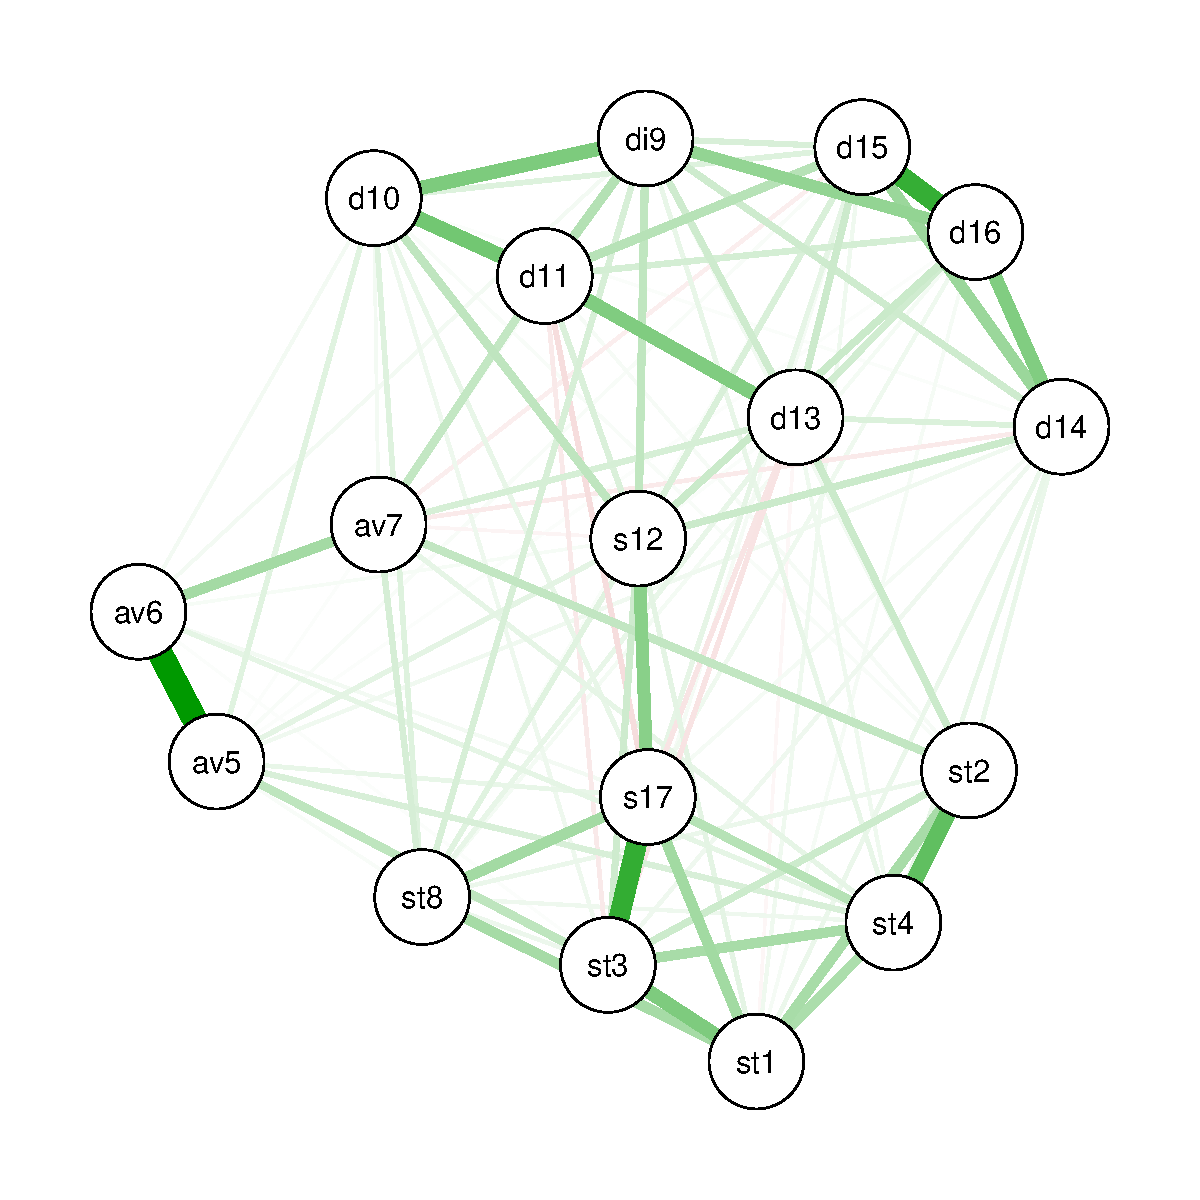
\includegraphics[width=\textwidth]{images/net_pcl5.pdf}
    \caption{Modeo a: red de los reactivos de estrés, evitación y distanciamiento. }
    \label{fig:netpcl5}
\end{subfigure}
\hfill
\begin{subfigure}{0.45\textwidth}
    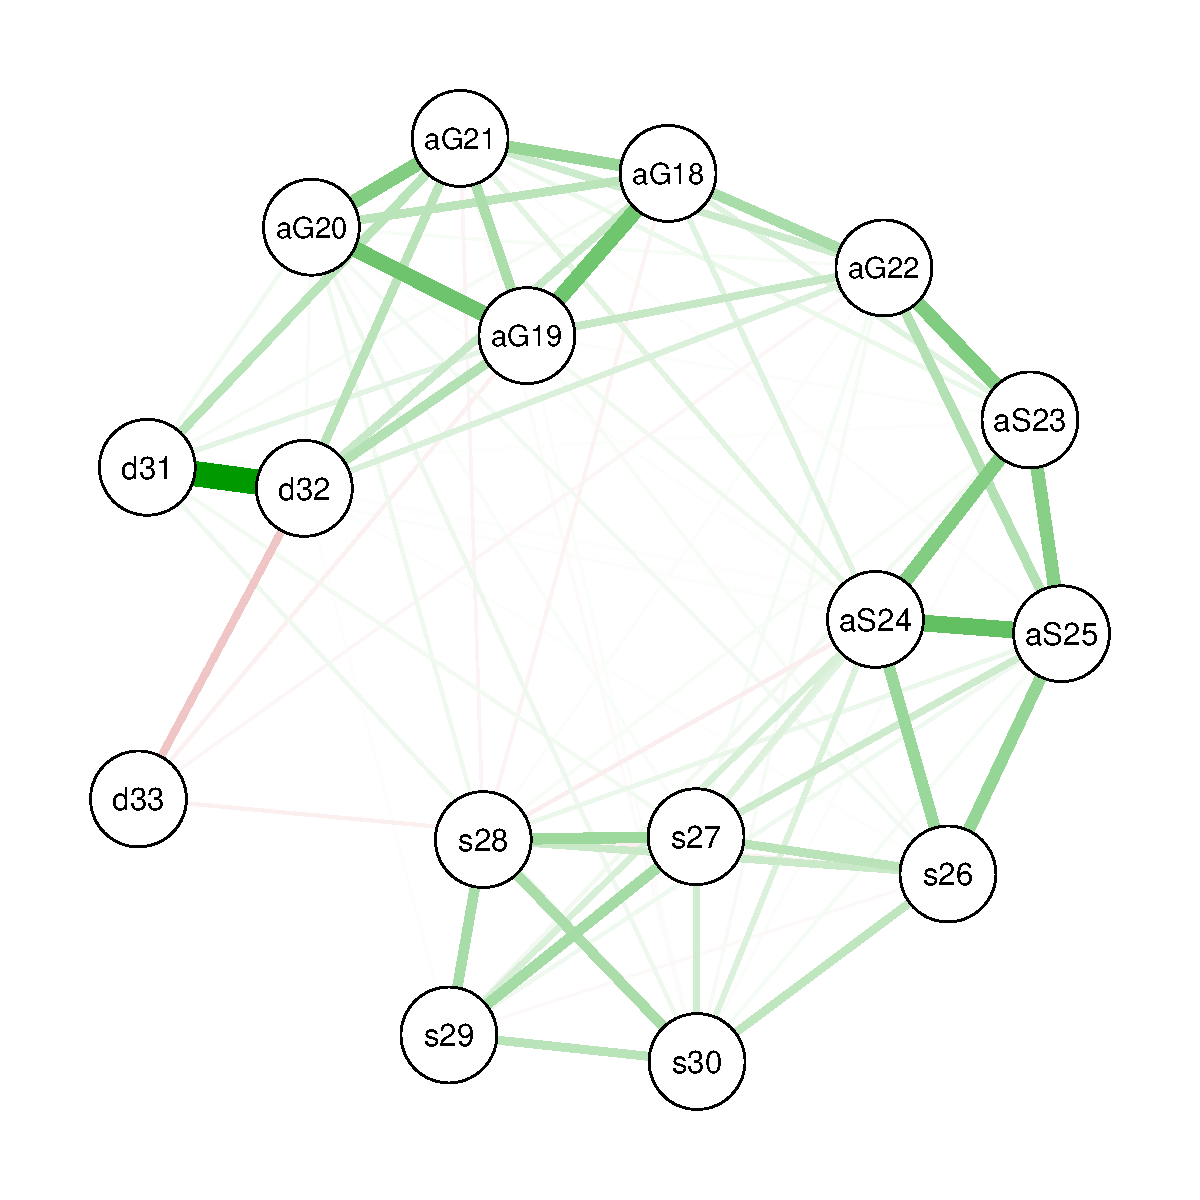
\includegraphics[width=\textwidth]{images/net_dean.pdf}
    \caption{Modelo b: red de los reactivos de ansiedad generalizada y por salud, somatización y depresión.}
    \label{fig:netdean}
\end{subfigure}
\hfill
\begin{subfigure}{0.7\textwidth}
    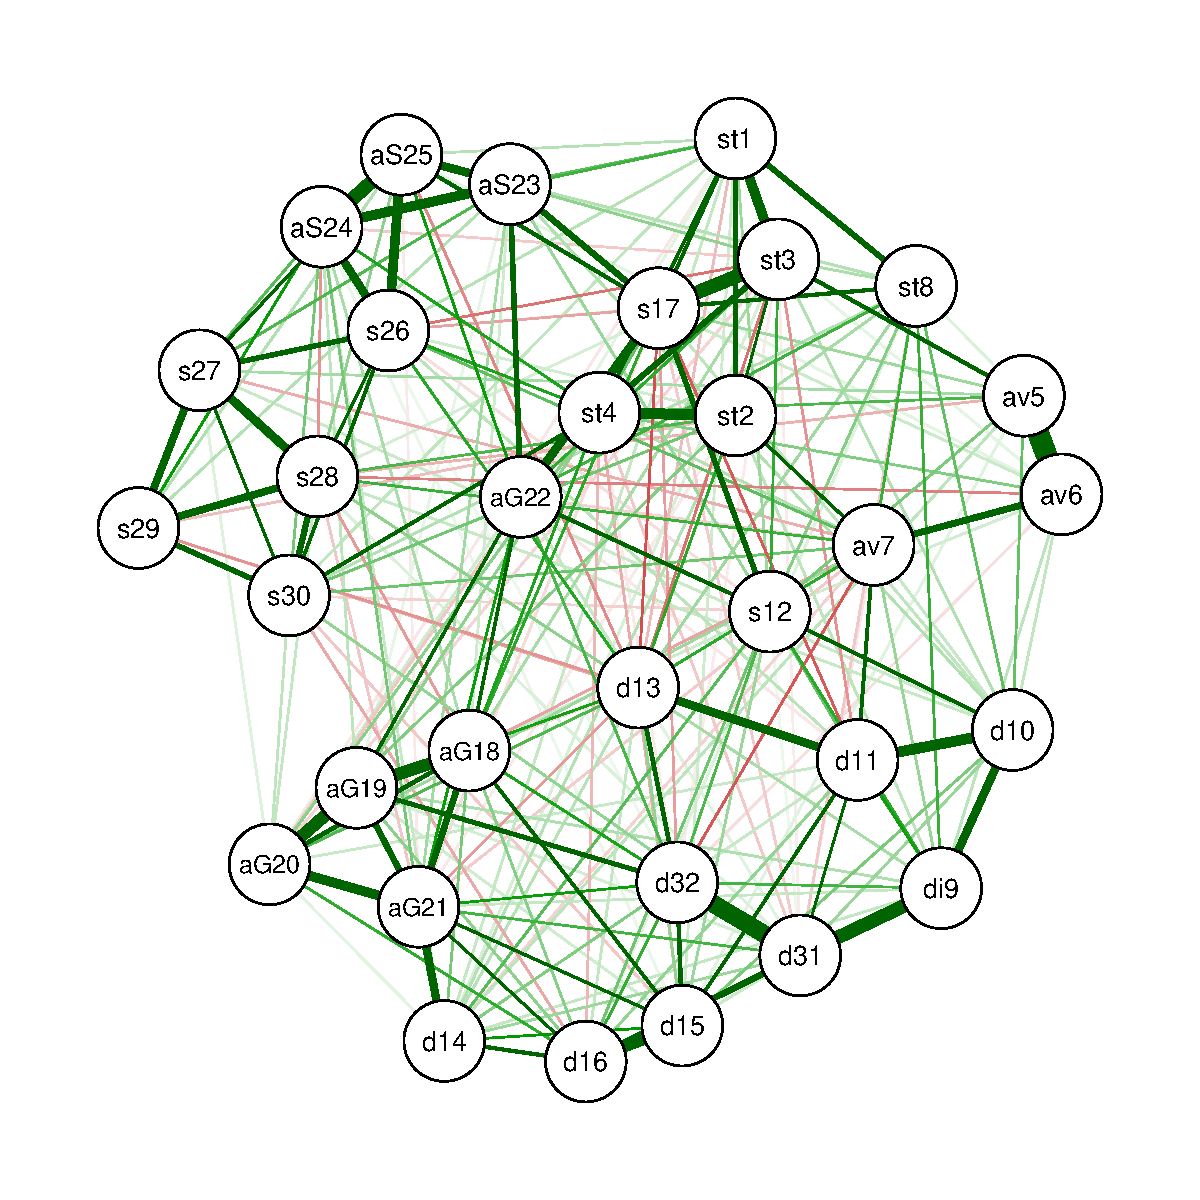
\includegraphics[width=\textwidth]{images/net_todo.pdf}
    \caption{Modelo c: red de todos los reactivos.}
    \label{fig:nettodos}
\end{subfigure}
\caption{Modelos de redes.}
\label{fig:nets}
\end{figure}

\newpage

La Figura \ref{fig:centra_ab} presenta las medidas de centralidad para los modelos a y b. Para este tipo de figura, los nodos están acomodados del que tiene más fuerza a los que tienen menor fuerza, de arriba hacia abajo. Para el panel a, el nodo con mayor fuerza es el st17 que habla de qué tan asustado se está por padecer la enfermedad, es decir, este es un reactivo importante que conecta directamente con otros nodos, seguido de los reactivos st3 y di11. Como se había mencionado anteriormente en el modelo a, el nodo st12 parece ser importante para interconectar con varios reactivos al mismo tiempo, y de hecho tiene las medidas de betweenneess y closeness más altas. Los nodos que tienen menor fuerza son los de evitación, y el st8 que habla de culpa por si alguien se enferma. Otro reactivo importante a analizar es el di10, que tiene betweennes bajo pero closeness alto. Esto indica que su interconexión muy cercana a otros nodos, pero no es un nodo que interconecte con más nodos más que con los que tiene cercanos, que son di9 y d11.

En cuanto a las medidas de centralidad del modelo b, se puede observar que el nodo con mayor fuerza es el as24 que se podría considerar un nodo importante en esta red. El nodo ag22, tiene las medidas de betweeness y closeness altas, de hecho, dentro de la red es el nodo que conecta más entre las dos principales agrupaciones. Por otro lado el nodo as23 tiene closeness alto pero no betweeness, lo cual tiene sentido pues es un nodo que está cercano a otros nodos importantes, pero no es único a la hora de interconectar con otras agrupaciones. 

La Figura \ref{fig:centra_todos} muestra las medidas de centralidad para el modelo c, que es el que tiene todos los reactivos. En esta red se observa que el nodo st17, que habla de estar asustado a padecer esta enfermedad, es de los que más fuerza tienen, además de que las medidas de betweenness y closeness también tiene valores muy altos. Le siguen los reactivos st3 y de32, siendo este último referente al constructo de depresión, que habla de sentirse decaído o deprimido. Esto es notable debido a que en el modelo b, este nodo no tenía tanta relevancia pero en este modelo alcanza el tercer lugar en fuerza. Adicionalmente, el nodo de ag22 tiene las medidas de betweenness y closeness altas, como lo había sido en el modelo b. Existen varios nodos que parecen no ser importantes en la red, y se refieren sobre todos a los de los síntomas de evitación, y los so29 y di14. 

\begin{figure}[ht!]
\centering
\begin{subfigure}{0.6\textwidth}
    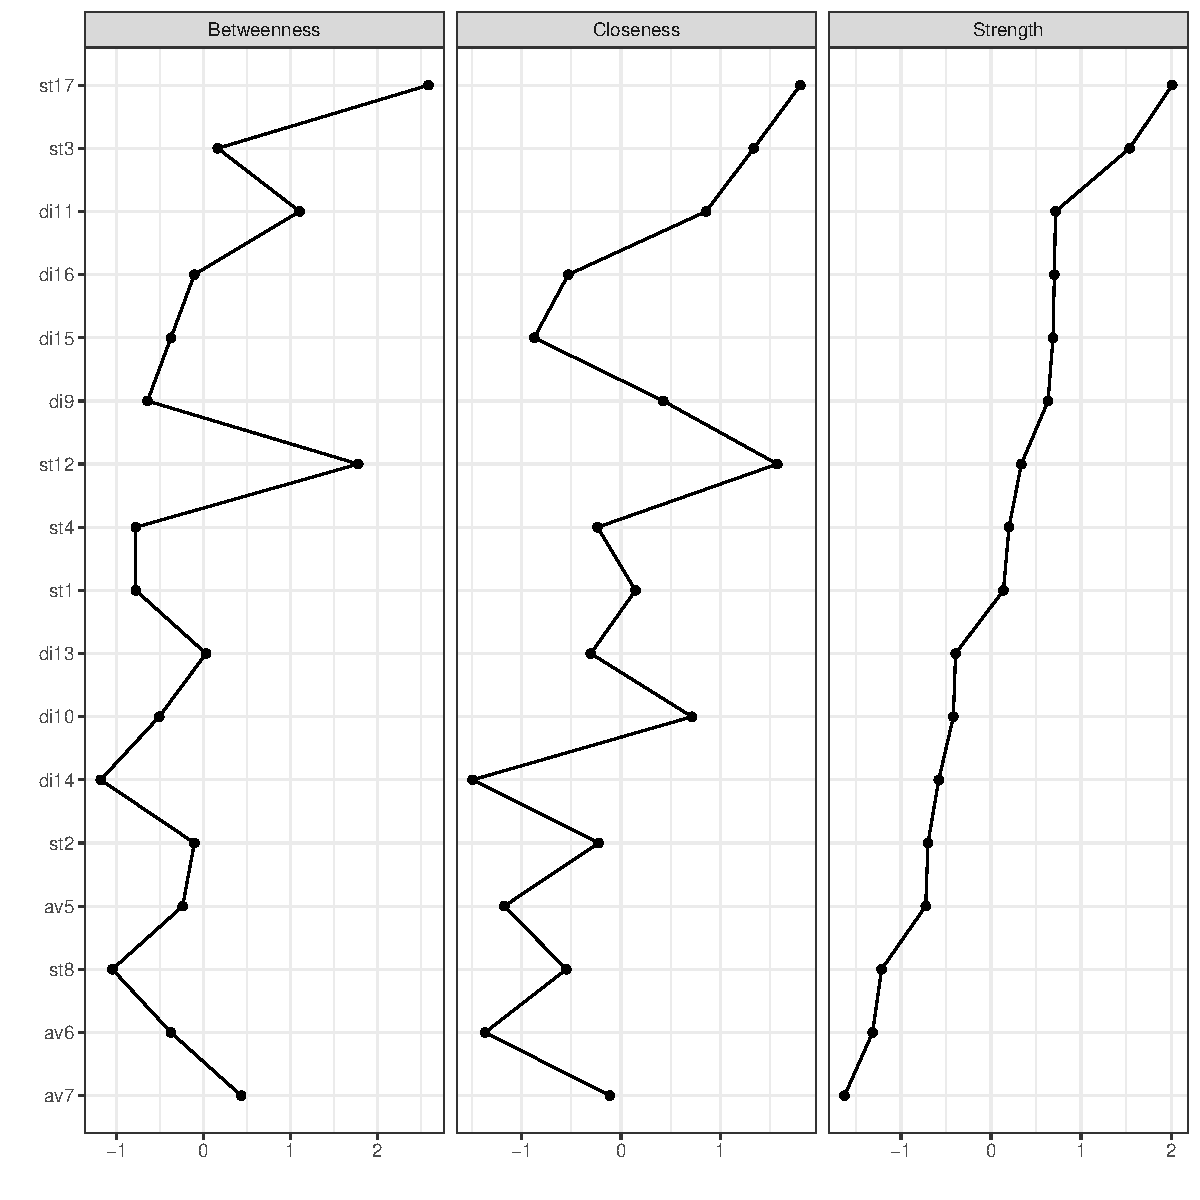
\includegraphics[width=\textwidth]{images/centrality_net_pcl5.pdf}
    \caption{Medidas de centralidad para el modelo a.}
    \label{fig:centrapcl5}
\end{subfigure}
\vfill
\begin{subfigure}{0.6\textwidth}
    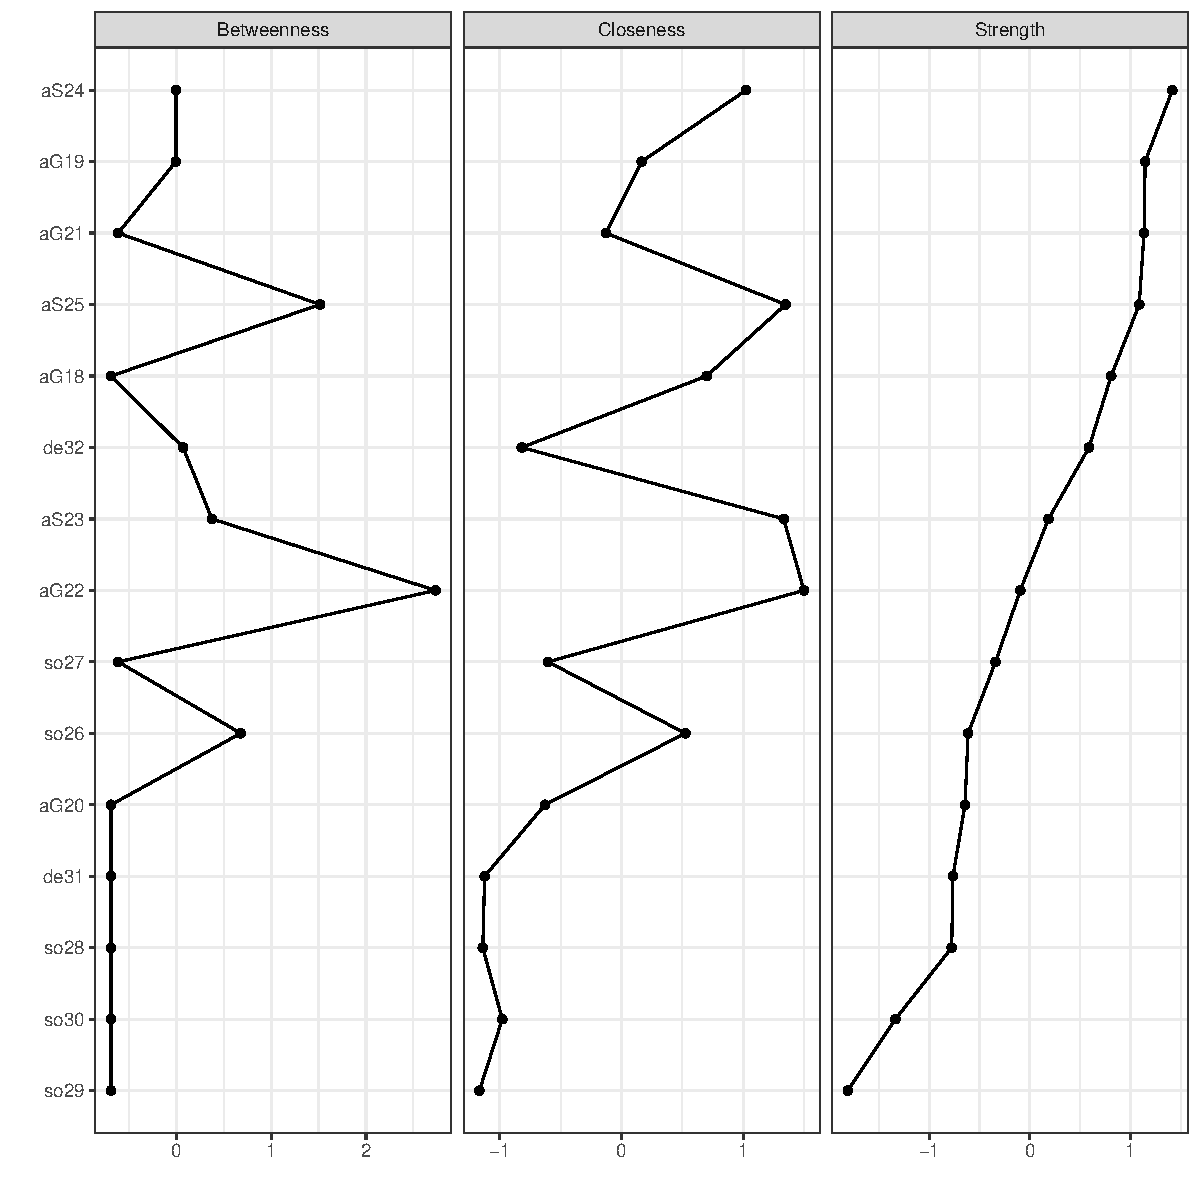
\includegraphics[width=\textwidth]{images/centrality_net_dean.pdf}
    \caption{Modelo b.}
    \label{fig:centradean}
\end{subfigure}
\caption{Medidas de centralidad para modelo a y b.}
\label{fig:centra_ab}
\end{figure}

\begin{figure}[ht!]
\centering
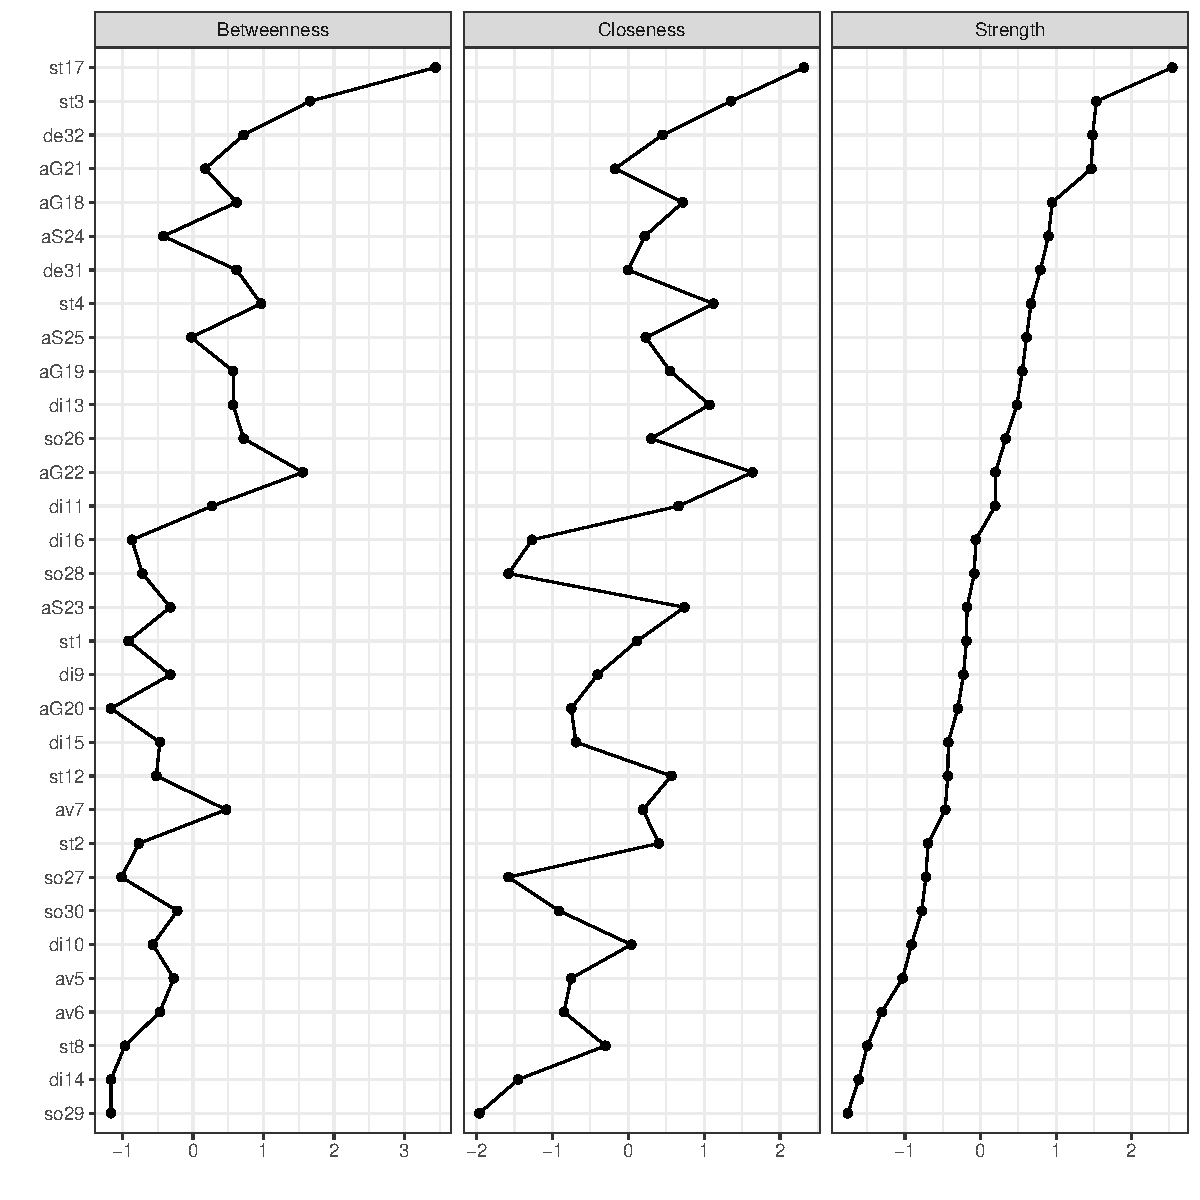
\includegraphics[scale=0.8]{images/centrality_net_todo.pdf}
\caption{Medidas de centralidad el modelo c.}
\label{fig:centra_todos}
\end{figure}

\clearpage

\newpage

\subsection{Precisión de pesos y estabilidad de medidas de centralidad}

Como se había comentado en la sección anterior es importante verificar tanto la precisión de los pesos de las aristas de cada modelo, así como la estabilidad de las medidas de centralidad. 

La Figura \ref{fig:intervalos} muestra los Intervalos de Confianza con bootstrap para los pesos de las aristas de los tres modelos. De manera general, en los tres gráficos se muestra que los intervalos son muy angostos para cada peso, además de que los valores de cada arista están muy separados unos de otros. Recordemos que en el eje $x$ están las aristas de mayor a menor peso, de arriba hacia abajo, por lo que tendremos tantos puntos como interconexiones estadísticamente relevantes dentro de la red. Por ejemplo en el panel a, el primer punto en la parte superior se encuentra la conexión más fuerte de la red, que parece ser entre los nodos st3 y s17. Para los tres modelos, en las conexiones más fuertes, podemos tener confianza de que los pesos de las aristas se pueden acercar al valor verdadero de esos pesos, por lo que se podrían considerar modelos estadísticos adecuados para tomar en cuenta.

La Figura \ref{fig:estabilidad} muestra la estabilidad de las medidas de centralidad con diferentes tamaños de muestra para los tres modelos. Para las tres redes se observa que la estabilidad en general es buena, pues no baja el promedio de correlación conforme se reduce el tamaño de muestra. El único detalle es que la medida de betweenness tiende a bajar un poco, sobre todo para el modelo b y un poco para el modelo c; sin embargo, esta baja no es pronunciada, por lo que podemos confiar en las medidas de centralidad que se obtuvieron de las redes. 

Por último, la Figura \ref{fig:sintodo} muestra un gráfico de diferencias significativas para la medida de fuerza de nodo del modelo c. En general se observa una gran presencia de negro entre los nodos, lo cual indica que la fuerza de los nodos es estadísticamente diferentes de los otros nodos. Por ejemplo, si observamos el nodo st17 tiene una fuerza de nodo estadísticamente diferente a todos los otros nodos, porque en todo su renglón solo hay presencia de negro. Caso contrario para la celda gris entre el nodo st12 y ag20 que nos indica que estos nodos no tienen una fuerza estadísticamente diferente una de otra. 

\begin{figure}[ht]
\centering
\begin{subfigure}{0.49\textwidth}
    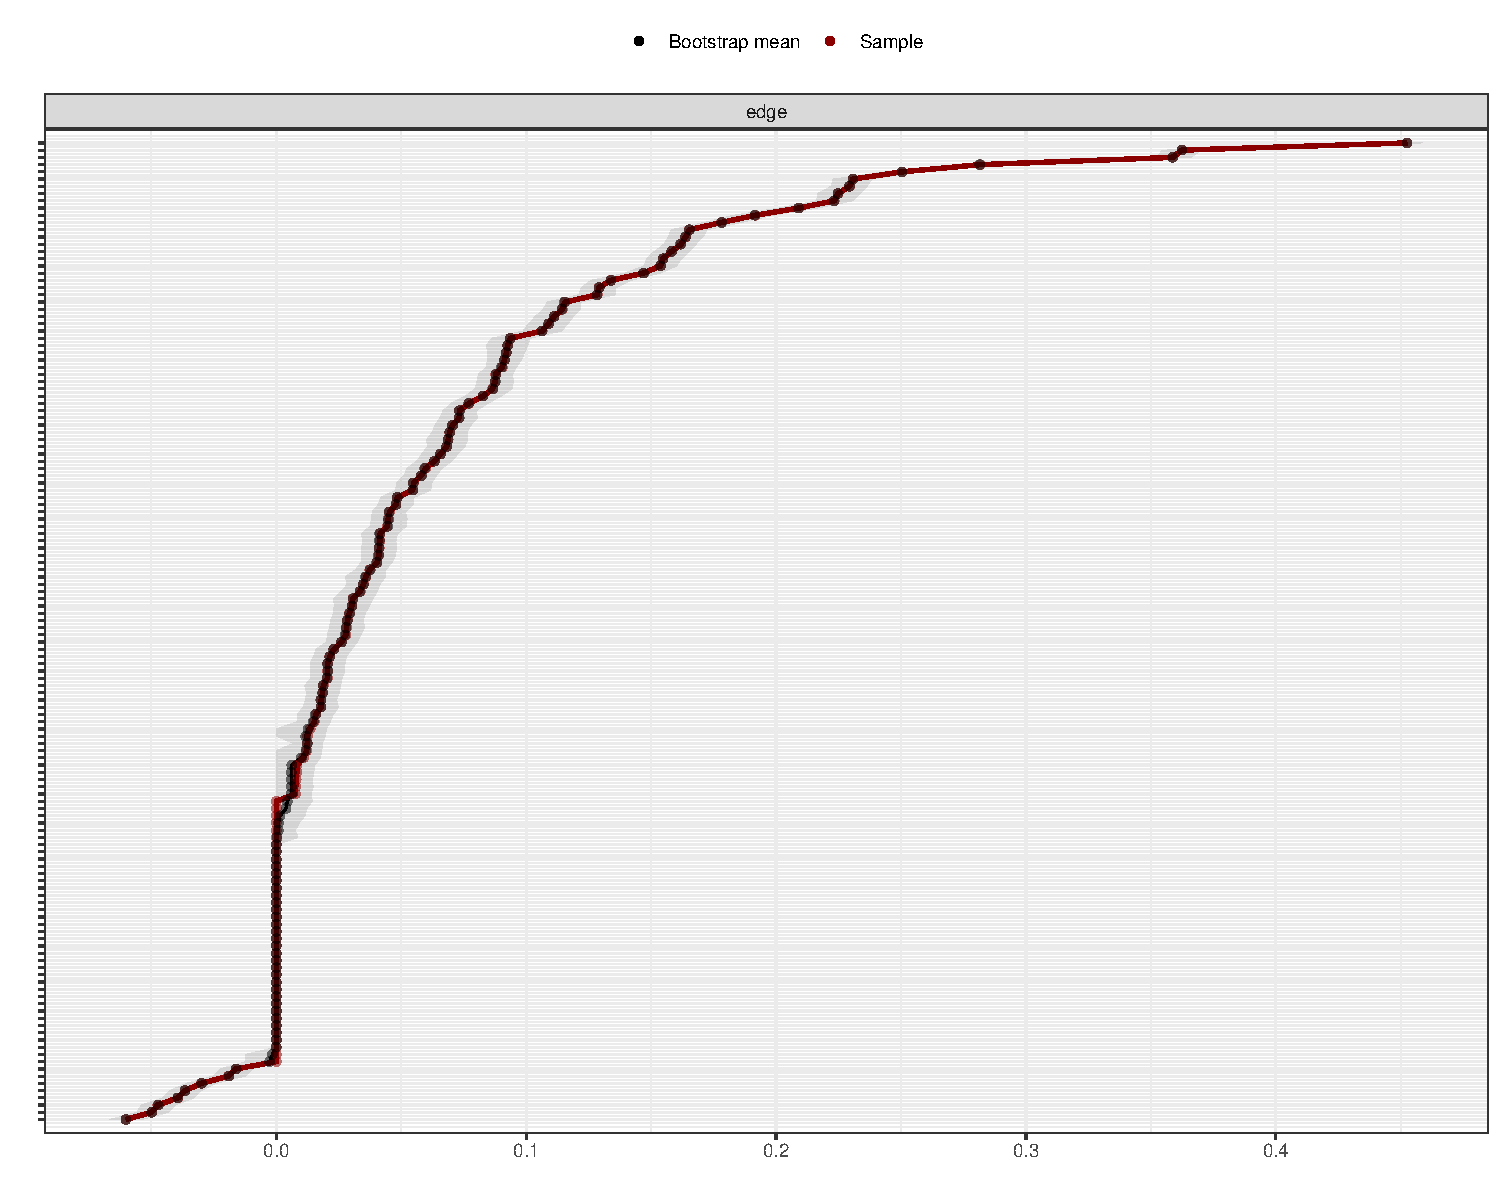
\includegraphics[width=\textwidth]{images/interval_pcl15.pdf}
    \caption{Intervalos de confianza para modelo a. }
    \label{fig:interval_pcl5}
\end{subfigure}
\begin{subfigure}{0.49\textwidth}
    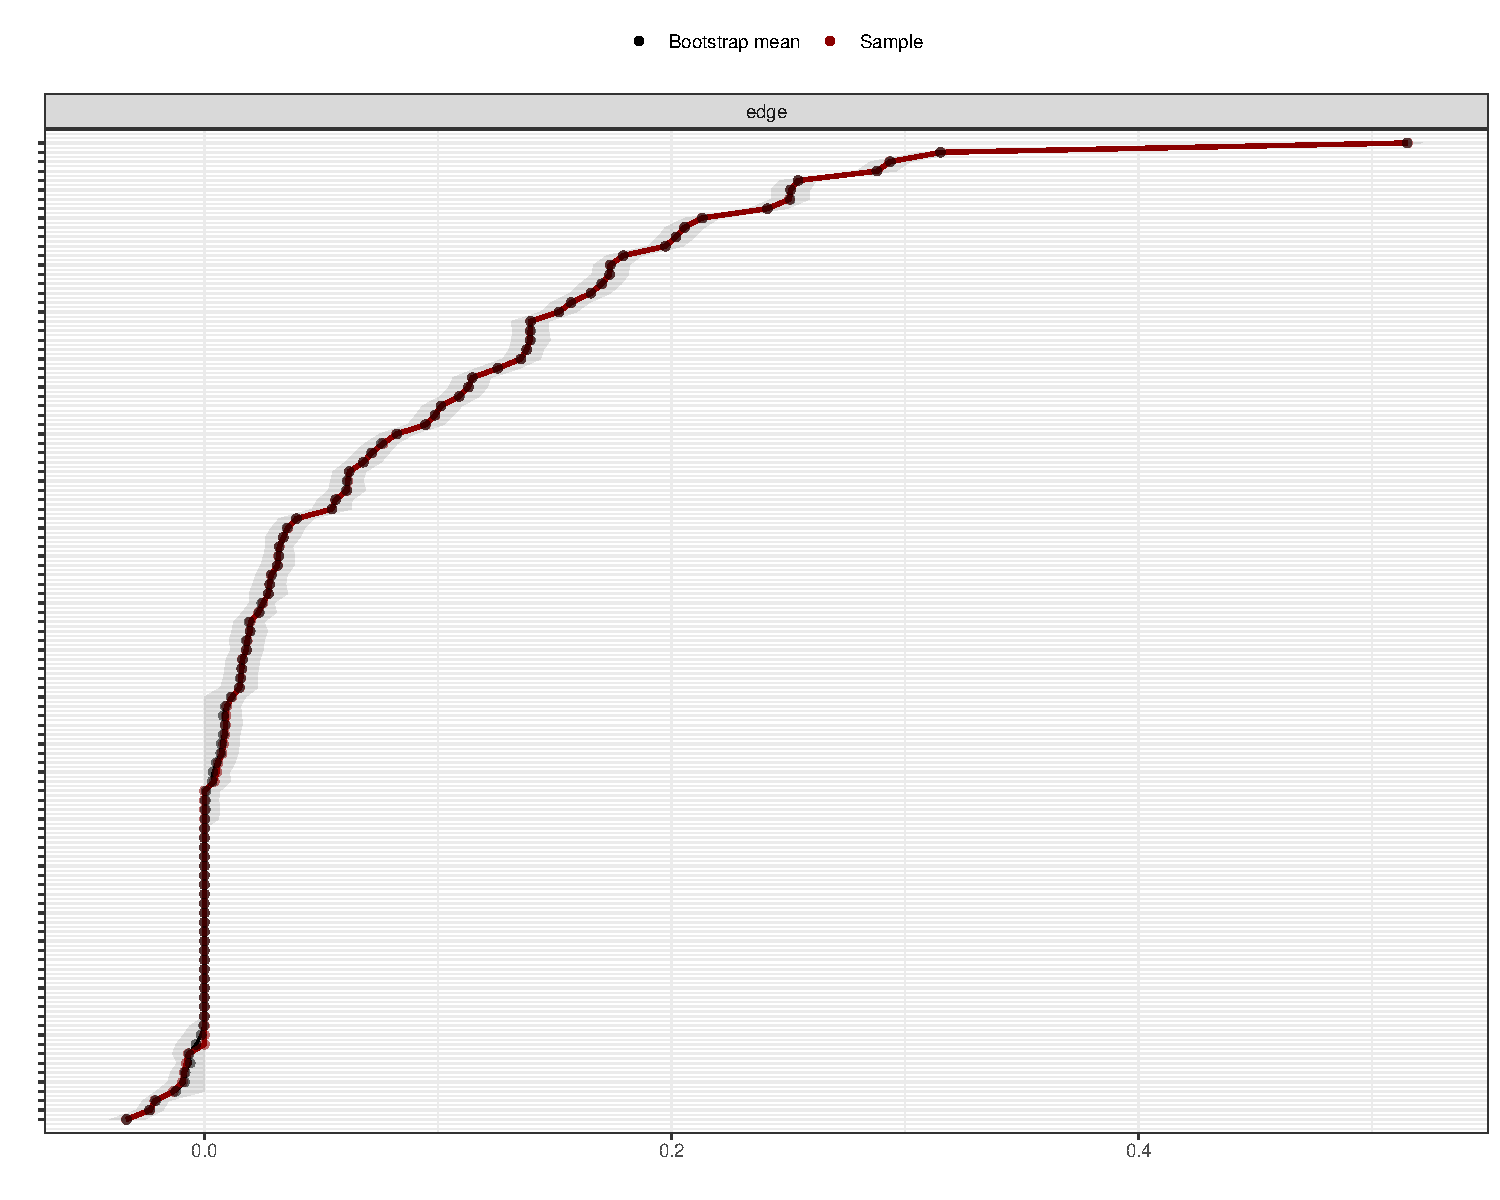
\includegraphics[width=\textwidth]{images/interval_dean.pdf}
  \caption{Intervalos de confianza para el modelo b. }
  \label{fig:interval_dean}
\end{subfigure}
\hfill
\begin{subfigure}{0.6\textwidth}
    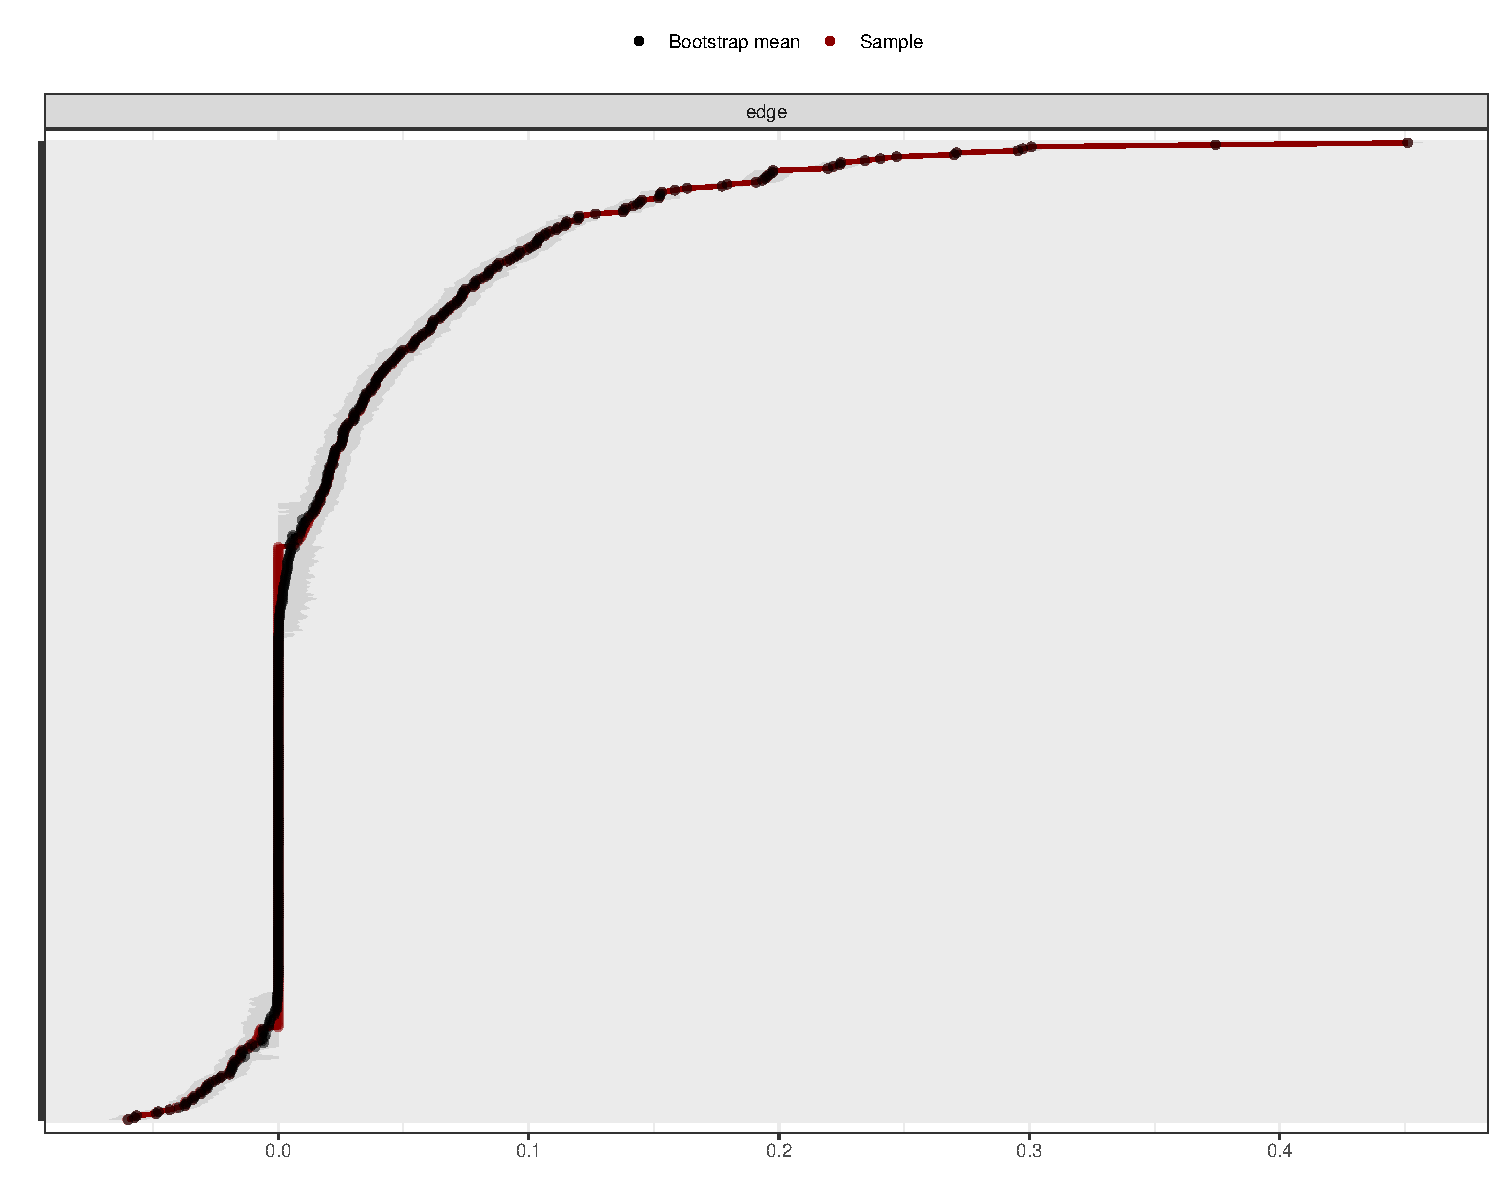
\includegraphics[width=\textwidth]{images/interval_todos.pdf}
    \caption{Intervalos de confianza para el modelo c.}
    \label{fig:interval_todo}
\end{subfigure}
\caption{Intervalos de Confianza de los modelos de redes.}
\label{fig:intervalos}
\end{figure}

\begin{figure}[ht]
\centering
\begin{subfigure}{0.49\textwidth}
    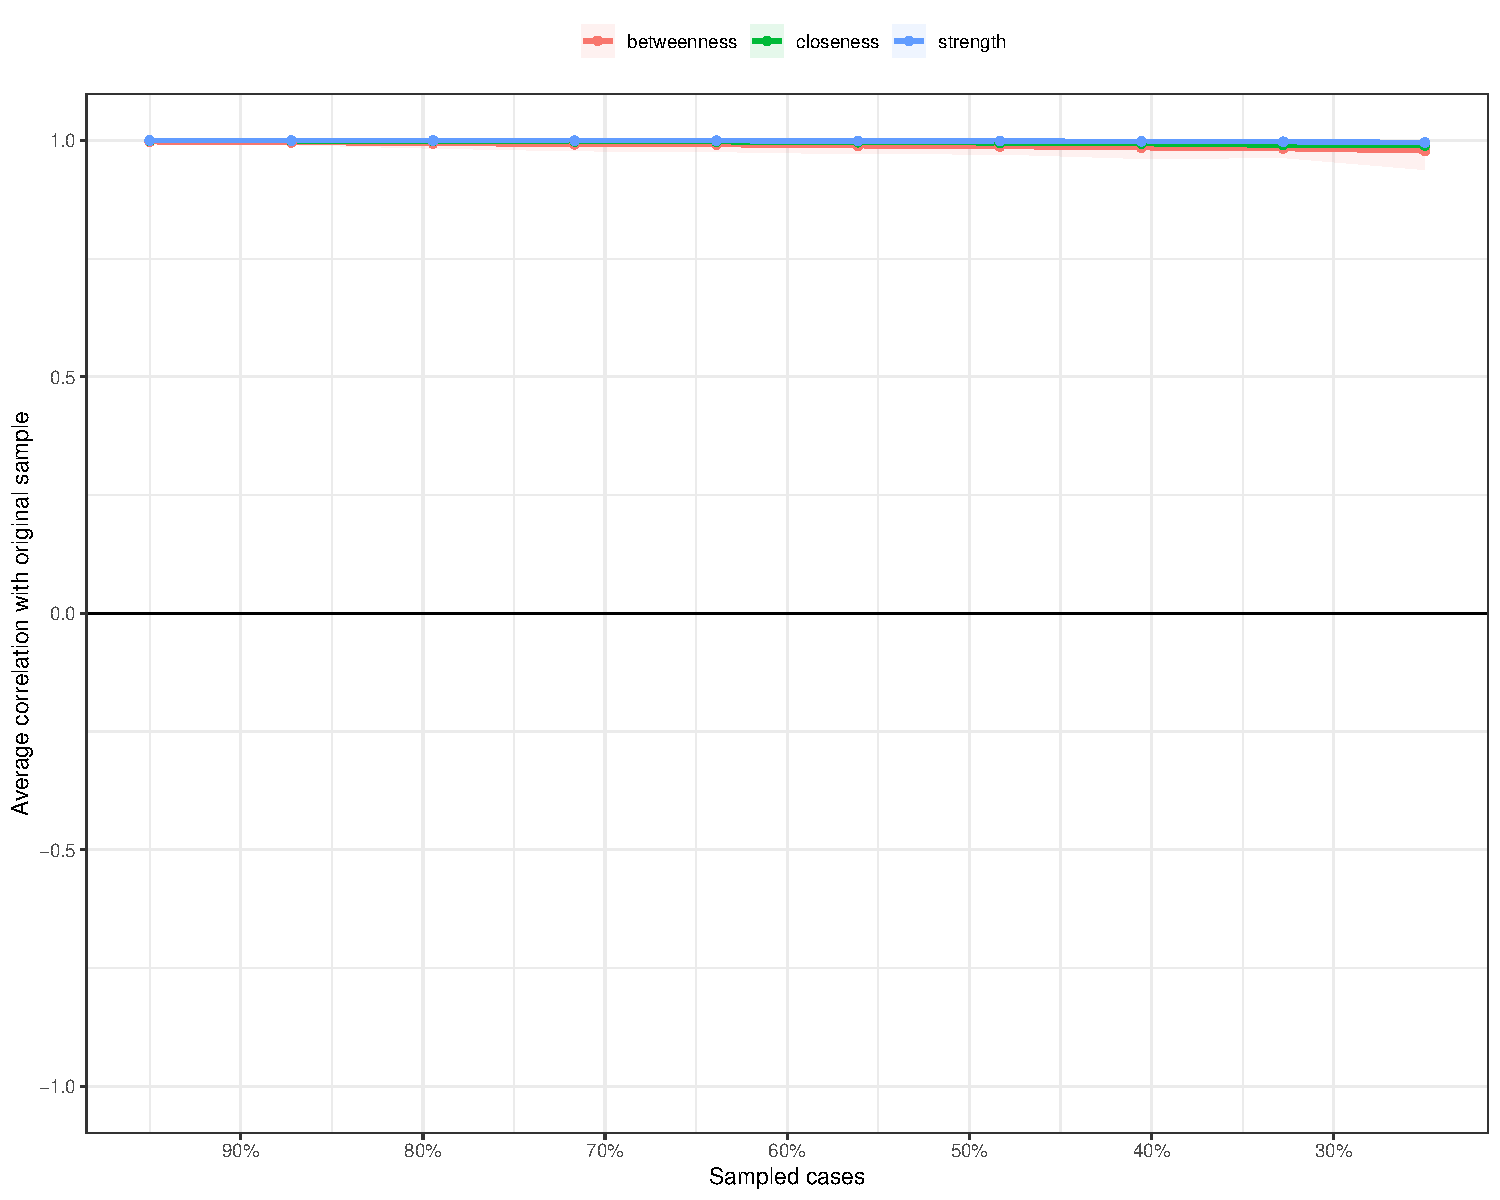
\includegraphics[width=\textwidth]{images/estability_pcl5.pdf}
\caption{Estabilidad de modelo a. }
\label{fig:estabilidad_pcl5}
\end{subfigure}
\begin{subfigure}{0.49\textwidth}
    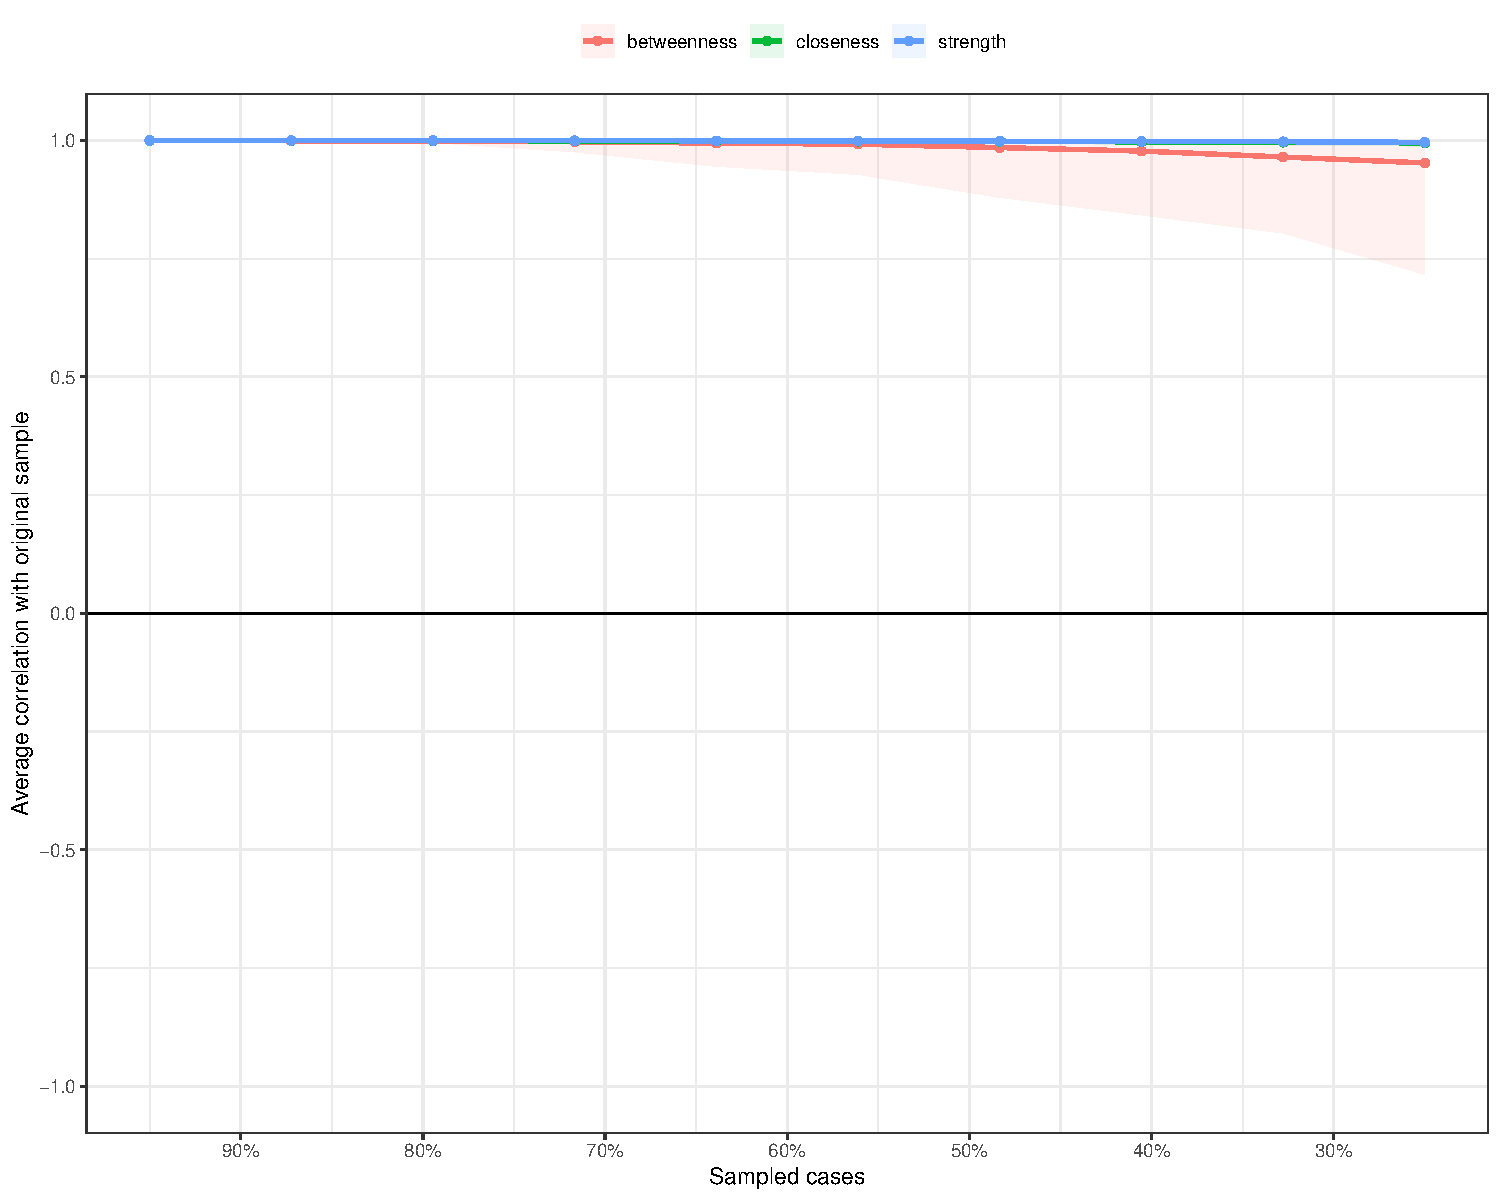
\includegraphics[width=\textwidth]{images/estability_dean.pdf}
\caption{Estabilidad de modelo b.}
\label{fig:estabilidad_dean}
\end{subfigure}
\hfill
\begin{subfigure}{0.6\textwidth}
    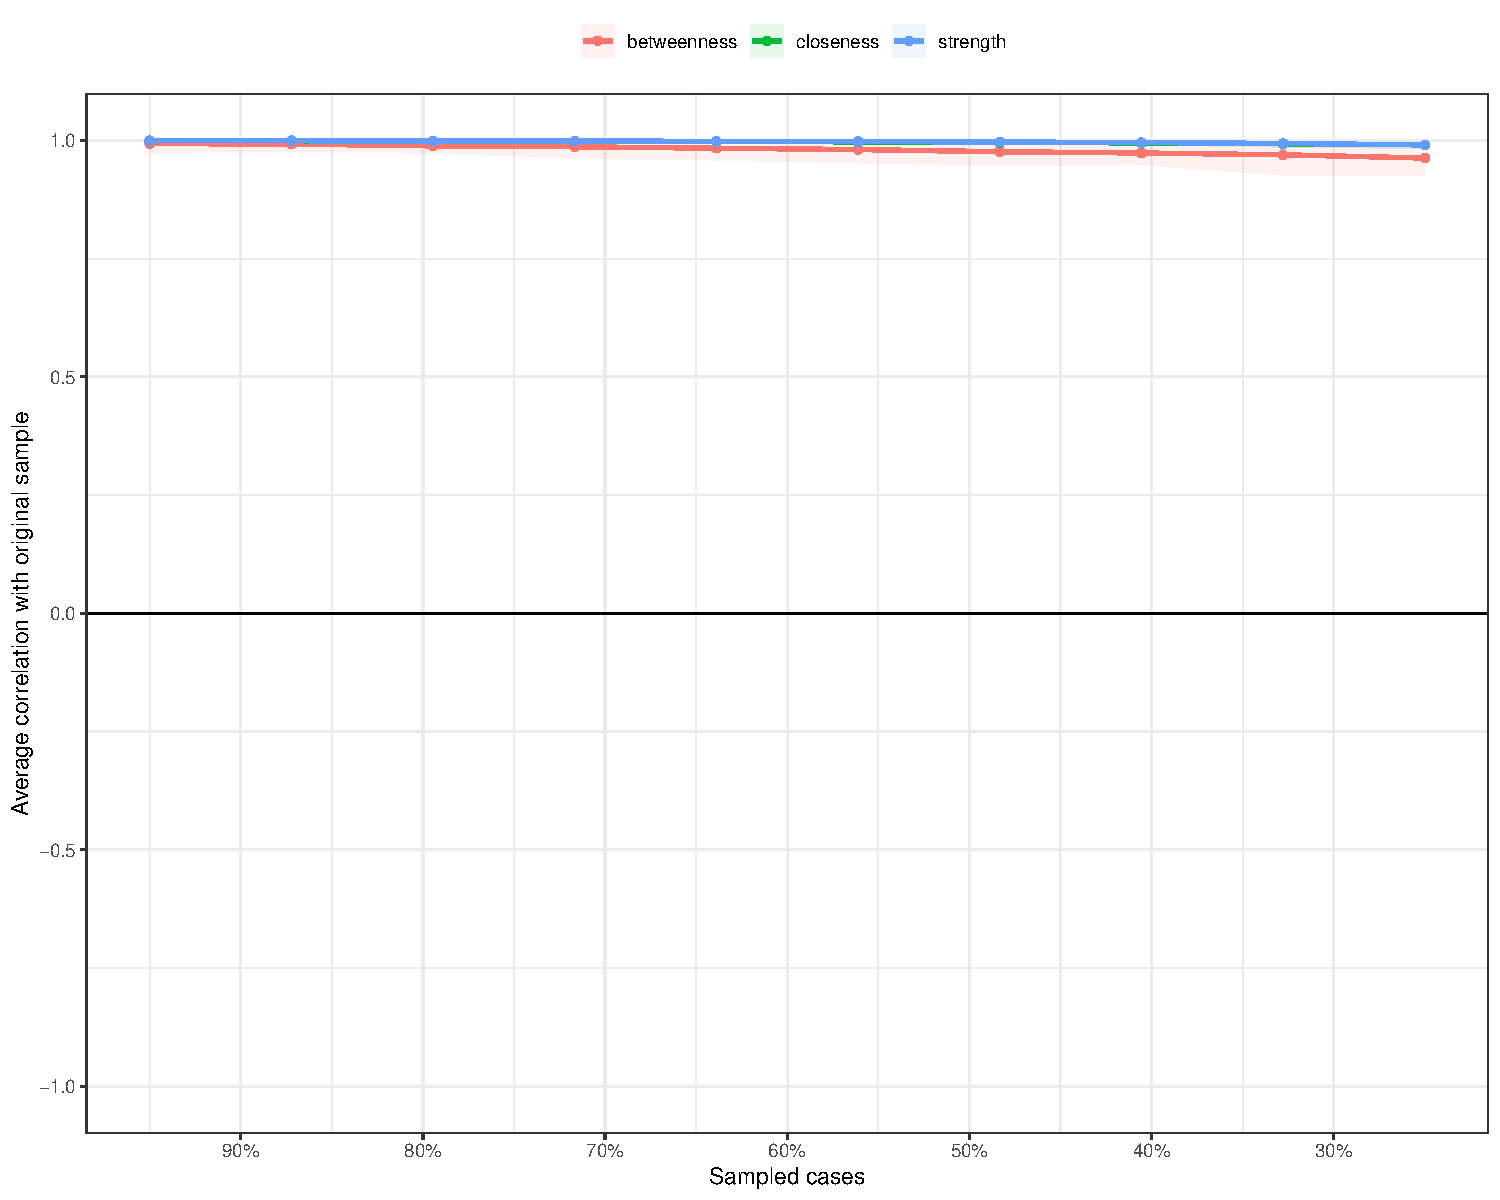
\includegraphics[width=\textwidth]{images/estability_todo.pdf}
    \caption{Estabilidad de modelo c.}
    \label{fig:estabilidad_todo}
\end{subfigure}
\caption{Estabilidad de las medidas de centralidad para los tres modelos.}
\label{fig:estabilidad}
\end{figure}


\begin{figure}[ht]
\centering
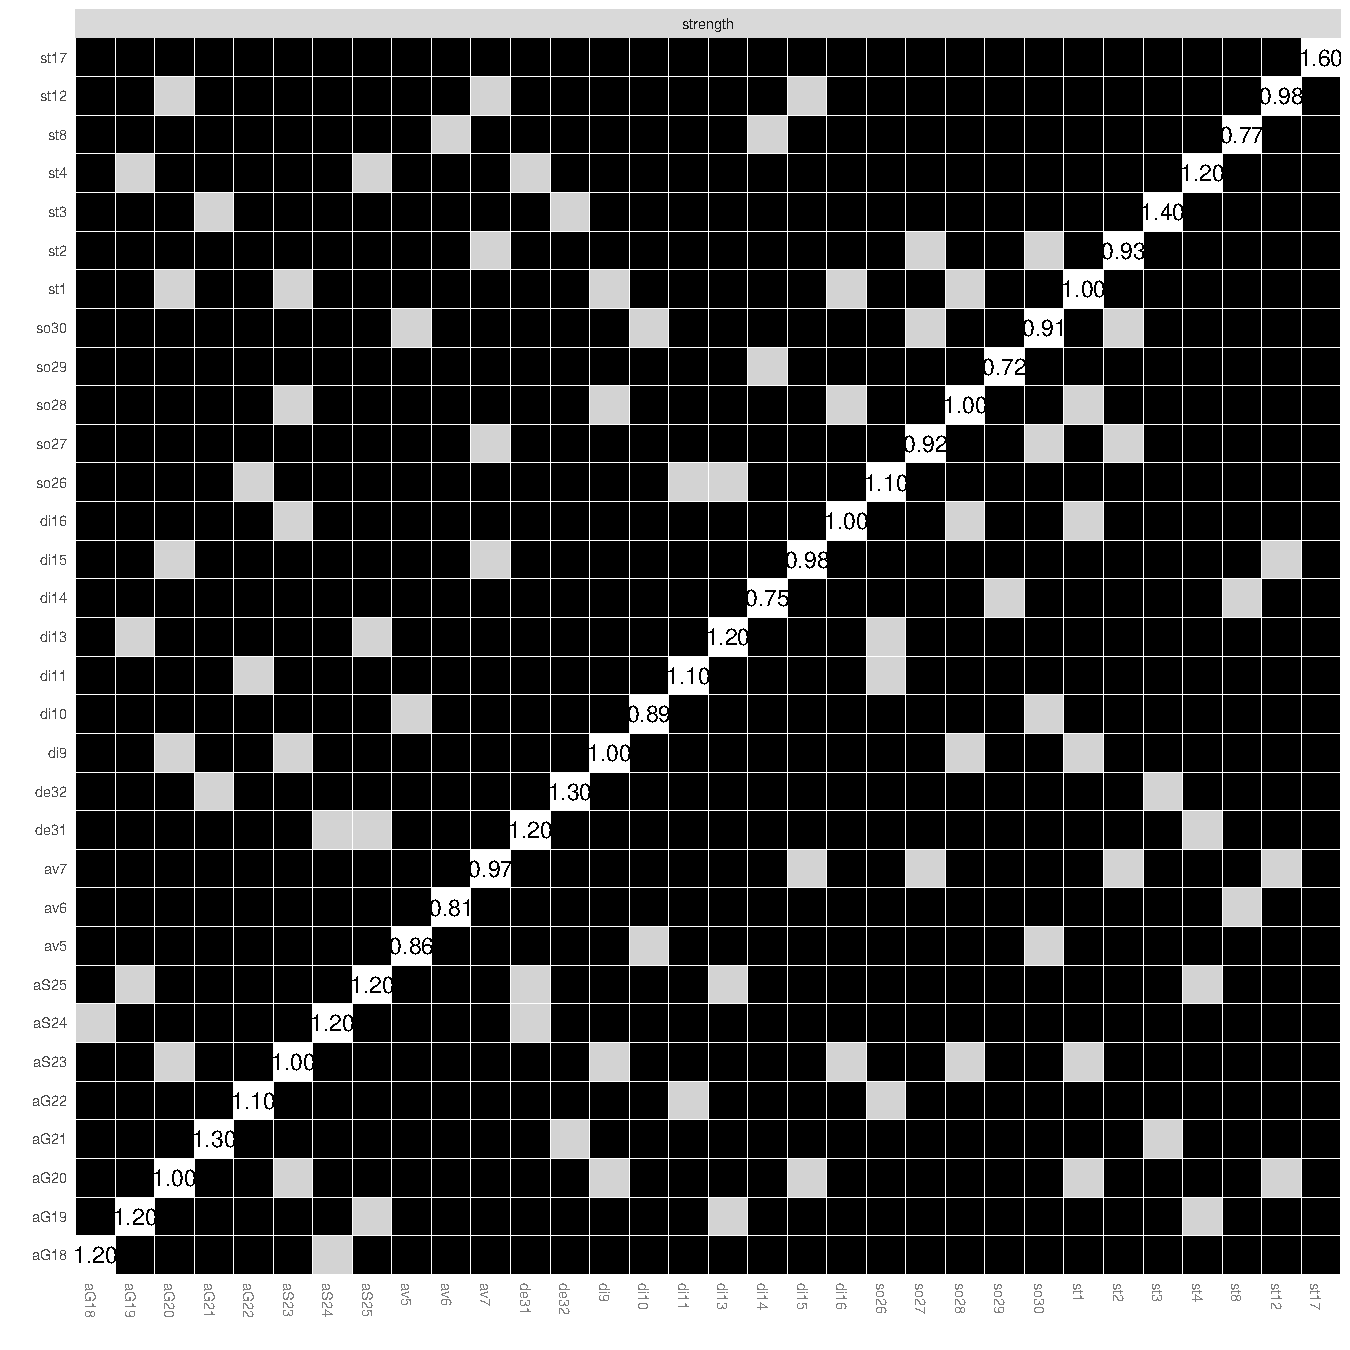
\includegraphics[scale=0.5]{images/signif_2i_todo.pdf}
\caption{Test de diferencias significativas entre los nodos del modelo c.}
\label{fig:sintodo}
\end{figure}

\clearpage

\subsection{Conclusiones}

El presente análisis es un preámbulo que muestra la riqueza que adhiere el análisis de redes psicológicas a la interpretación de resultados de la base de riesgos de enfermedades mentales a partir del Covid-19. Se dice que es preámbulo debido a que los presentes resultados son un modelo base que todavía se tiene que analizar y explorar a más detalle. A pesar de ser un modelo base, se encontraron resultados muy relevantes que se pueden extrapolar a otras preguntas de investigación que nos ayuden a ver cómo interactúan los síntomas, a ver cuáles son las otras interdependencias que ayudan a desarrollar algún desorden mental, a ver su co-morbilidad de síntomas con otros constructos, y ver cuáles son los síntomas que sirven de puente entre los diferentes desórdenes, entre otras cosas \citep{fried2017mental, haslbeck2017predictable}.

Los siguientes pasos son plantear diferentes modelos de redes en función de preguntas de investigación bien establecidas y comparando variables, por ejemplo, ver las redes de los usuarios que enfermaron de covid versus lo que no, etc. También corresponde comparar y ver el funcionamiento de estos resultados, con los resultados que se han obtenido de los análisis tradicionalmente hechos para este tipo de datos.

% ##########  NOTAS DE ARTICULOSSS
% 
% Mental disorder as networks of problems.
% 
% 
% Conceptualización de redes en psicopatología. 
% 
% Un desorden metal se puede ver como un sistema de síntomas interactuando. Desde esta perspectiva, hay un juego causal entre los síntomas que constituyen al desorden mental. Por ejemplo, Desorden de Depresión Mayor, los síntomas son: tristesa, anhedonia, fatiga, insomio, problemas de concentración e ideación suicida. A partir de estos síntomas se puede n ver relaciones causales entre los problemas, por ejemplo: fatiga -> insomio -> problemas de concentración o tritesa -> anhedonia -> ideas suicidas. 
% 
% Comorbilidad
% 
% Es común que existan al mismo tiempo, múltiples desordenes mentales. Tradicionalmente, la comorbilidad de desórdenes mentales se entienden como diferentes desórdenes, mientras que la perspectiva de redes tiene de hipótesis que éstos ocurren debido a una interacicón entre síntomas. En este sentido, comorbilidad se da cuando hay un puente entre dos síntomas que vienen de diferentes desórdenes. 
% 
% Una implicación del punto de vista de redes es que los diagnósticos pueden co-ocurrir como una función del número de síntomas compartidos. Esta implicación no se comparte necesariamente desde el punto de vista tradiicional. 
% 
% Ver los desórdenes a un nivel más a partir de síntomas, revelaría un poco del mecanismo de comorbilidad. 
% 
% Predicción
% 
% Una de las áreas más importantes de investigación clínica es la predicción de psicopatologías desde el comienzo para así, desarrollar intervenciones clínicas tempranas. Por lo que la literatura en predicción se enfoca en dos aspectos 1) las llamadas señales de alerta temprana que pueden indicar la próxima aparición de psicopatología para un paciente específico, y 2) las características de redes a nivel grupal que pueden ayudar a predecir el curso futuro de la psicopatología. 
% 
% 
% 
% Señales de alerta temprana
% 
% Existen áreas en ciencias en los cuáles sistemas complejos se pueden comprender-estudiar adecuadamente. Uno de las características más importantes de sistemas complejos es que se pueden mostrar fases de transiciones. Lo interesantes es que justo andes de una fase de transición de un estado a otro, y sistema despliega señales de alerta temprana. Específicamente, dichas transiciones se preceden por un fenómeno referido como alentamiento crítico, que significa que le lleva más tiempo a us sistema a recuperarse de perturbaciones. Esto se refleja por el hecho de que los sistemas se hacen más predecibles por sus estados previos: cuando se acercan a una transición, la dinámica se alenta. 
% 
% 
% 
% Centralidad
% 
% 
% El número de conexiones que tiene un nodo (síntoma). Si tienes un síntoma que tiene más conexiones entonces hay más posibilidades de que eso desarrolle otros síntomas, pero si desarrollas un nodo más periférico no será tan grande la posibilidad. El grado de centralidad se puede entender cómo la cuantificación de la importancia de un nodo en una red. Otras medidas son closeness and betweenness. 
% 
% 
% ###########
% 
% How predictable are symptoms in psychopathological networks? 
% 
% 
% La previsibilidad es el grado en el cual un nodo dado puede ser predicho por los demás nodos en la red. 
% 
% ############
% 
% Latent Variable Models and Networks:
% 
% Comparación entre modelos, aunque nada quedó realmente definido, está interesante el artículo porque ven la equivalencia entre los modelos, además, expresan la dificultad de hacer comparaciones entre éstos debido a que sus predicciones no se pueden comparar. Lo leí sólo por encima y sólo la discusión, merece una revisada a detalle.


\clearpage
\bibliography{bibtex}

\end{document}
